
% Default to the notebook output style

    


% Inherit from the specified cell style.




    
\documentclass[11pt]{article}

    
    
    \usepackage[T1]{fontenc}
    % Nicer default font (+ math font) than Computer Modern for most use cases
    \usepackage{mathpazo}

    % Basic figure setup, for now with no caption control since it's done
    % automatically by Pandoc (which extracts ![](path) syntax from Markdown).
    \usepackage{graphicx}
    % We will generate all images so they have a width \maxwidth. This means
    % that they will get their normal width if they fit onto the page, but
    % are scaled down if they would overflow the margins.
    \makeatletter
    \def\maxwidth{\ifdim\Gin@nat@width>\linewidth\linewidth
    \else\Gin@nat@width\fi}
    \makeatother
    \let\Oldincludegraphics\includegraphics
    % Set max figure width to be 80% of text width, for now hardcoded.
    \renewcommand{\includegraphics}[1]{\Oldincludegraphics[width=.8\maxwidth]{#1}}
    % Ensure that by default, figures have no caption (until we provide a
    % proper Figure object with a Caption API and a way to capture that
    % in the conversion process - todo).
    \usepackage{caption}
    \DeclareCaptionLabelFormat{nolabel}{}
    \captionsetup{labelformat=nolabel}

    \usepackage{adjustbox} % Used to constrain images to a maximum size 
    \usepackage{xcolor} % Allow colors to be defined
    \usepackage{enumerate} % Needed for markdown enumerations to work
    \usepackage{geometry} % Used to adjust the document margins
    \usepackage{amsmath} % Equations
    \usepackage{amssymb} % Equations
    \usepackage{textcomp} % defines textquotesingle
    % Hack from http://tex.stackexchange.com/a/47451/13684:
    \AtBeginDocument{%
        \def\PYZsq{\textquotesingle}% Upright quotes in Pygmentized code
    }
    \usepackage{upquote} % Upright quotes for verbatim code
    \usepackage{eurosym} % defines \euro
    \usepackage[mathletters]{ucs} % Extended unicode (utf-8) support
    \usepackage[utf8x]{inputenc} % Allow utf-8 characters in the tex document
    \usepackage{fancyvrb} % verbatim replacement that allows latex
    \usepackage{grffile} % extends the file name processing of package graphics 
                         % to support a larger range 
    % The hyperref package gives us a pdf with properly built
    % internal navigation ('pdf bookmarks' for the table of contents,
    % internal cross-reference links, web links for URLs, etc.)
    \usepackage{hyperref}
    \usepackage{longtable} % longtable support required by pandoc >1.10
    \usepackage{booktabs}  % table support for pandoc > 1.12.2
    \usepackage[inline]{enumitem} % IRkernel/repr support (it uses the enumerate* environment)
    \usepackage[normalem]{ulem} % ulem is needed to support strikethroughs (\sout)
                                % normalem makes italics be italics, not underlines
    

    
    
    % Colors for the hyperref package
    \definecolor{urlcolor}{rgb}{0,.145,.698}
    \definecolor{linkcolor}{rgb}{.71,0.21,0.01}
    \definecolor{citecolor}{rgb}{.12,.54,.11}

    % ANSI colors
    \definecolor{ansi-black}{HTML}{3E424D}
    \definecolor{ansi-black-intense}{HTML}{282C36}
    \definecolor{ansi-red}{HTML}{E75C58}
    \definecolor{ansi-red-intense}{HTML}{B22B31}
    \definecolor{ansi-green}{HTML}{00A250}
    \definecolor{ansi-green-intense}{HTML}{007427}
    \definecolor{ansi-yellow}{HTML}{DDB62B}
    \definecolor{ansi-yellow-intense}{HTML}{B27D12}
    \definecolor{ansi-blue}{HTML}{208FFB}
    \definecolor{ansi-blue-intense}{HTML}{0065CA}
    \definecolor{ansi-magenta}{HTML}{D160C4}
    \definecolor{ansi-magenta-intense}{HTML}{A03196}
    \definecolor{ansi-cyan}{HTML}{60C6C8}
    \definecolor{ansi-cyan-intense}{HTML}{258F8F}
    \definecolor{ansi-white}{HTML}{C5C1B4}
    \definecolor{ansi-white-intense}{HTML}{A1A6B2}

    % commands and environments needed by pandoc snippets
    % extracted from the output of `pandoc -s`
    \providecommand{\tightlist}{%
      \setlength{\itemsep}{0pt}\setlength{\parskip}{0pt}}
    \DefineVerbatimEnvironment{Highlighting}{Verbatim}{commandchars=\\\{\}}
    % Add ',fontsize=\small' for more characters per line
    \newenvironment{Shaded}{}{}
    \newcommand{\KeywordTok}[1]{\textcolor[rgb]{0.00,0.44,0.13}{\textbf{{#1}}}}
    \newcommand{\DataTypeTok}[1]{\textcolor[rgb]{0.56,0.13,0.00}{{#1}}}
    \newcommand{\DecValTok}[1]{\textcolor[rgb]{0.25,0.63,0.44}{{#1}}}
    \newcommand{\BaseNTok}[1]{\textcolor[rgb]{0.25,0.63,0.44}{{#1}}}
    \newcommand{\FloatTok}[1]{\textcolor[rgb]{0.25,0.63,0.44}{{#1}}}
    \newcommand{\CharTok}[1]{\textcolor[rgb]{0.25,0.44,0.63}{{#1}}}
    \newcommand{\StringTok}[1]{\textcolor[rgb]{0.25,0.44,0.63}{{#1}}}
    \newcommand{\CommentTok}[1]{\textcolor[rgb]{0.38,0.63,0.69}{\textit{{#1}}}}
    \newcommand{\OtherTok}[1]{\textcolor[rgb]{0.00,0.44,0.13}{{#1}}}
    \newcommand{\AlertTok}[1]{\textcolor[rgb]{1.00,0.00,0.00}{\textbf{{#1}}}}
    \newcommand{\FunctionTok}[1]{\textcolor[rgb]{0.02,0.16,0.49}{{#1}}}
    \newcommand{\RegionMarkerTok}[1]{{#1}}
    \newcommand{\ErrorTok}[1]{\textcolor[rgb]{1.00,0.00,0.00}{\textbf{{#1}}}}
    \newcommand{\NormalTok}[1]{{#1}}
    
    % Additional commands for more recent versions of Pandoc
    \newcommand{\ConstantTok}[1]{\textcolor[rgb]{0.53,0.00,0.00}{{#1}}}
    \newcommand{\SpecialCharTok}[1]{\textcolor[rgb]{0.25,0.44,0.63}{{#1}}}
    \newcommand{\VerbatimStringTok}[1]{\textcolor[rgb]{0.25,0.44,0.63}{{#1}}}
    \newcommand{\SpecialStringTok}[1]{\textcolor[rgb]{0.73,0.40,0.53}{{#1}}}
    \newcommand{\ImportTok}[1]{{#1}}
    \newcommand{\DocumentationTok}[1]{\textcolor[rgb]{0.73,0.13,0.13}{\textit{{#1}}}}
    \newcommand{\AnnotationTok}[1]{\textcolor[rgb]{0.38,0.63,0.69}{\textbf{\textit{{#1}}}}}
    \newcommand{\CommentVarTok}[1]{\textcolor[rgb]{0.38,0.63,0.69}{\textbf{\textit{{#1}}}}}
    \newcommand{\VariableTok}[1]{\textcolor[rgb]{0.10,0.09,0.49}{{#1}}}
    \newcommand{\ControlFlowTok}[1]{\textcolor[rgb]{0.00,0.44,0.13}{\textbf{{#1}}}}
    \newcommand{\OperatorTok}[1]{\textcolor[rgb]{0.40,0.40,0.40}{{#1}}}
    \newcommand{\BuiltInTok}[1]{{#1}}
    \newcommand{\ExtensionTok}[1]{{#1}}
    \newcommand{\PreprocessorTok}[1]{\textcolor[rgb]{0.74,0.48,0.00}{{#1}}}
    \newcommand{\AttributeTok}[1]{\textcolor[rgb]{0.49,0.56,0.16}{{#1}}}
    \newcommand{\InformationTok}[1]{\textcolor[rgb]{0.38,0.63,0.69}{\textbf{\textit{{#1}}}}}
    \newcommand{\WarningTok}[1]{\textcolor[rgb]{0.38,0.63,0.69}{\textbf{\textit{{#1}}}}}
    
    
    % Define a nice break command that doesn't care if a line doesn't already
    % exist.
    \def\br{\hspace*{\fill} \\* }
    % Math Jax compatability definitions
    \def\gt{>}
    \def\lt{<}
    % Document parameters
    \title{cnn\_rnn\_models}
    
    
    

    % Pygments definitions
    
\makeatletter
\def\PY@reset{\let\PY@it=\relax \let\PY@bf=\relax%
    \let\PY@ul=\relax \let\PY@tc=\relax%
    \let\PY@bc=\relax \let\PY@ff=\relax}
\def\PY@tok#1{\csname PY@tok@#1\endcsname}
\def\PY@toks#1+{\ifx\relax#1\empty\else%
    \PY@tok{#1}\expandafter\PY@toks\fi}
\def\PY@do#1{\PY@bc{\PY@tc{\PY@ul{%
    \PY@it{\PY@bf{\PY@ff{#1}}}}}}}
\def\PY#1#2{\PY@reset\PY@toks#1+\relax+\PY@do{#2}}

\expandafter\def\csname PY@tok@w\endcsname{\def\PY@tc##1{\textcolor[rgb]{0.73,0.73,0.73}{##1}}}
\expandafter\def\csname PY@tok@c\endcsname{\let\PY@it=\textit\def\PY@tc##1{\textcolor[rgb]{0.25,0.50,0.50}{##1}}}
\expandafter\def\csname PY@tok@cp\endcsname{\def\PY@tc##1{\textcolor[rgb]{0.74,0.48,0.00}{##1}}}
\expandafter\def\csname PY@tok@k\endcsname{\let\PY@bf=\textbf\def\PY@tc##1{\textcolor[rgb]{0.00,0.50,0.00}{##1}}}
\expandafter\def\csname PY@tok@kp\endcsname{\def\PY@tc##1{\textcolor[rgb]{0.00,0.50,0.00}{##1}}}
\expandafter\def\csname PY@tok@kt\endcsname{\def\PY@tc##1{\textcolor[rgb]{0.69,0.00,0.25}{##1}}}
\expandafter\def\csname PY@tok@o\endcsname{\def\PY@tc##1{\textcolor[rgb]{0.40,0.40,0.40}{##1}}}
\expandafter\def\csname PY@tok@ow\endcsname{\let\PY@bf=\textbf\def\PY@tc##1{\textcolor[rgb]{0.67,0.13,1.00}{##1}}}
\expandafter\def\csname PY@tok@nb\endcsname{\def\PY@tc##1{\textcolor[rgb]{0.00,0.50,0.00}{##1}}}
\expandafter\def\csname PY@tok@nf\endcsname{\def\PY@tc##1{\textcolor[rgb]{0.00,0.00,1.00}{##1}}}
\expandafter\def\csname PY@tok@nc\endcsname{\let\PY@bf=\textbf\def\PY@tc##1{\textcolor[rgb]{0.00,0.00,1.00}{##1}}}
\expandafter\def\csname PY@tok@nn\endcsname{\let\PY@bf=\textbf\def\PY@tc##1{\textcolor[rgb]{0.00,0.00,1.00}{##1}}}
\expandafter\def\csname PY@tok@ne\endcsname{\let\PY@bf=\textbf\def\PY@tc##1{\textcolor[rgb]{0.82,0.25,0.23}{##1}}}
\expandafter\def\csname PY@tok@nv\endcsname{\def\PY@tc##1{\textcolor[rgb]{0.10,0.09,0.49}{##1}}}
\expandafter\def\csname PY@tok@no\endcsname{\def\PY@tc##1{\textcolor[rgb]{0.53,0.00,0.00}{##1}}}
\expandafter\def\csname PY@tok@nl\endcsname{\def\PY@tc##1{\textcolor[rgb]{0.63,0.63,0.00}{##1}}}
\expandafter\def\csname PY@tok@ni\endcsname{\let\PY@bf=\textbf\def\PY@tc##1{\textcolor[rgb]{0.60,0.60,0.60}{##1}}}
\expandafter\def\csname PY@tok@na\endcsname{\def\PY@tc##1{\textcolor[rgb]{0.49,0.56,0.16}{##1}}}
\expandafter\def\csname PY@tok@nt\endcsname{\let\PY@bf=\textbf\def\PY@tc##1{\textcolor[rgb]{0.00,0.50,0.00}{##1}}}
\expandafter\def\csname PY@tok@nd\endcsname{\def\PY@tc##1{\textcolor[rgb]{0.67,0.13,1.00}{##1}}}
\expandafter\def\csname PY@tok@s\endcsname{\def\PY@tc##1{\textcolor[rgb]{0.73,0.13,0.13}{##1}}}
\expandafter\def\csname PY@tok@sd\endcsname{\let\PY@it=\textit\def\PY@tc##1{\textcolor[rgb]{0.73,0.13,0.13}{##1}}}
\expandafter\def\csname PY@tok@si\endcsname{\let\PY@bf=\textbf\def\PY@tc##1{\textcolor[rgb]{0.73,0.40,0.53}{##1}}}
\expandafter\def\csname PY@tok@se\endcsname{\let\PY@bf=\textbf\def\PY@tc##1{\textcolor[rgb]{0.73,0.40,0.13}{##1}}}
\expandafter\def\csname PY@tok@sr\endcsname{\def\PY@tc##1{\textcolor[rgb]{0.73,0.40,0.53}{##1}}}
\expandafter\def\csname PY@tok@ss\endcsname{\def\PY@tc##1{\textcolor[rgb]{0.10,0.09,0.49}{##1}}}
\expandafter\def\csname PY@tok@sx\endcsname{\def\PY@tc##1{\textcolor[rgb]{0.00,0.50,0.00}{##1}}}
\expandafter\def\csname PY@tok@m\endcsname{\def\PY@tc##1{\textcolor[rgb]{0.40,0.40,0.40}{##1}}}
\expandafter\def\csname PY@tok@gh\endcsname{\let\PY@bf=\textbf\def\PY@tc##1{\textcolor[rgb]{0.00,0.00,0.50}{##1}}}
\expandafter\def\csname PY@tok@gu\endcsname{\let\PY@bf=\textbf\def\PY@tc##1{\textcolor[rgb]{0.50,0.00,0.50}{##1}}}
\expandafter\def\csname PY@tok@gd\endcsname{\def\PY@tc##1{\textcolor[rgb]{0.63,0.00,0.00}{##1}}}
\expandafter\def\csname PY@tok@gi\endcsname{\def\PY@tc##1{\textcolor[rgb]{0.00,0.63,0.00}{##1}}}
\expandafter\def\csname PY@tok@gr\endcsname{\def\PY@tc##1{\textcolor[rgb]{1.00,0.00,0.00}{##1}}}
\expandafter\def\csname PY@tok@ge\endcsname{\let\PY@it=\textit}
\expandafter\def\csname PY@tok@gs\endcsname{\let\PY@bf=\textbf}
\expandafter\def\csname PY@tok@gp\endcsname{\let\PY@bf=\textbf\def\PY@tc##1{\textcolor[rgb]{0.00,0.00,0.50}{##1}}}
\expandafter\def\csname PY@tok@go\endcsname{\def\PY@tc##1{\textcolor[rgb]{0.53,0.53,0.53}{##1}}}
\expandafter\def\csname PY@tok@gt\endcsname{\def\PY@tc##1{\textcolor[rgb]{0.00,0.27,0.87}{##1}}}
\expandafter\def\csname PY@tok@err\endcsname{\def\PY@bc##1{\setlength{\fboxsep}{0pt}\fcolorbox[rgb]{1.00,0.00,0.00}{1,1,1}{\strut ##1}}}
\expandafter\def\csname PY@tok@kc\endcsname{\let\PY@bf=\textbf\def\PY@tc##1{\textcolor[rgb]{0.00,0.50,0.00}{##1}}}
\expandafter\def\csname PY@tok@kd\endcsname{\let\PY@bf=\textbf\def\PY@tc##1{\textcolor[rgb]{0.00,0.50,0.00}{##1}}}
\expandafter\def\csname PY@tok@kn\endcsname{\let\PY@bf=\textbf\def\PY@tc##1{\textcolor[rgb]{0.00,0.50,0.00}{##1}}}
\expandafter\def\csname PY@tok@kr\endcsname{\let\PY@bf=\textbf\def\PY@tc##1{\textcolor[rgb]{0.00,0.50,0.00}{##1}}}
\expandafter\def\csname PY@tok@bp\endcsname{\def\PY@tc##1{\textcolor[rgb]{0.00,0.50,0.00}{##1}}}
\expandafter\def\csname PY@tok@fm\endcsname{\def\PY@tc##1{\textcolor[rgb]{0.00,0.00,1.00}{##1}}}
\expandafter\def\csname PY@tok@vc\endcsname{\def\PY@tc##1{\textcolor[rgb]{0.10,0.09,0.49}{##1}}}
\expandafter\def\csname PY@tok@vg\endcsname{\def\PY@tc##1{\textcolor[rgb]{0.10,0.09,0.49}{##1}}}
\expandafter\def\csname PY@tok@vi\endcsname{\def\PY@tc##1{\textcolor[rgb]{0.10,0.09,0.49}{##1}}}
\expandafter\def\csname PY@tok@vm\endcsname{\def\PY@tc##1{\textcolor[rgb]{0.10,0.09,0.49}{##1}}}
\expandafter\def\csname PY@tok@sa\endcsname{\def\PY@tc##1{\textcolor[rgb]{0.73,0.13,0.13}{##1}}}
\expandafter\def\csname PY@tok@sb\endcsname{\def\PY@tc##1{\textcolor[rgb]{0.73,0.13,0.13}{##1}}}
\expandafter\def\csname PY@tok@sc\endcsname{\def\PY@tc##1{\textcolor[rgb]{0.73,0.13,0.13}{##1}}}
\expandafter\def\csname PY@tok@dl\endcsname{\def\PY@tc##1{\textcolor[rgb]{0.73,0.13,0.13}{##1}}}
\expandafter\def\csname PY@tok@s2\endcsname{\def\PY@tc##1{\textcolor[rgb]{0.73,0.13,0.13}{##1}}}
\expandafter\def\csname PY@tok@sh\endcsname{\def\PY@tc##1{\textcolor[rgb]{0.73,0.13,0.13}{##1}}}
\expandafter\def\csname PY@tok@s1\endcsname{\def\PY@tc##1{\textcolor[rgb]{0.73,0.13,0.13}{##1}}}
\expandafter\def\csname PY@tok@mb\endcsname{\def\PY@tc##1{\textcolor[rgb]{0.40,0.40,0.40}{##1}}}
\expandafter\def\csname PY@tok@mf\endcsname{\def\PY@tc##1{\textcolor[rgb]{0.40,0.40,0.40}{##1}}}
\expandafter\def\csname PY@tok@mh\endcsname{\def\PY@tc##1{\textcolor[rgb]{0.40,0.40,0.40}{##1}}}
\expandafter\def\csname PY@tok@mi\endcsname{\def\PY@tc##1{\textcolor[rgb]{0.40,0.40,0.40}{##1}}}
\expandafter\def\csname PY@tok@il\endcsname{\def\PY@tc##1{\textcolor[rgb]{0.40,0.40,0.40}{##1}}}
\expandafter\def\csname PY@tok@mo\endcsname{\def\PY@tc##1{\textcolor[rgb]{0.40,0.40,0.40}{##1}}}
\expandafter\def\csname PY@tok@ch\endcsname{\let\PY@it=\textit\def\PY@tc##1{\textcolor[rgb]{0.25,0.50,0.50}{##1}}}
\expandafter\def\csname PY@tok@cm\endcsname{\let\PY@it=\textit\def\PY@tc##1{\textcolor[rgb]{0.25,0.50,0.50}{##1}}}
\expandafter\def\csname PY@tok@cpf\endcsname{\let\PY@it=\textit\def\PY@tc##1{\textcolor[rgb]{0.25,0.50,0.50}{##1}}}
\expandafter\def\csname PY@tok@c1\endcsname{\let\PY@it=\textit\def\PY@tc##1{\textcolor[rgb]{0.25,0.50,0.50}{##1}}}
\expandafter\def\csname PY@tok@cs\endcsname{\let\PY@it=\textit\def\PY@tc##1{\textcolor[rgb]{0.25,0.50,0.50}{##1}}}

\def\PYZbs{\char`\\}
\def\PYZus{\char`\_}
\def\PYZob{\char`\{}
\def\PYZcb{\char`\}}
\def\PYZca{\char`\^}
\def\PYZam{\char`\&}
\def\PYZlt{\char`\<}
\def\PYZgt{\char`\>}
\def\PYZsh{\char`\#}
\def\PYZpc{\char`\%}
\def\PYZdl{\char`\$}
\def\PYZhy{\char`\-}
\def\PYZsq{\char`\'}
\def\PYZdq{\char`\"}
\def\PYZti{\char`\~}
% for compatibility with earlier versions
\def\PYZat{@}
\def\PYZlb{[}
\def\PYZrb{]}
\makeatother


    % Exact colors from NB
    \definecolor{incolor}{rgb}{0.0, 0.0, 0.5}
    \definecolor{outcolor}{rgb}{0.545, 0.0, 0.0}



    
    % Prevent overflowing lines due to hard-to-break entities
    \sloppy 
    % Setup hyperref package
    \hypersetup{
      breaklinks=true,  % so long urls are correctly broken across lines
      colorlinks=true,
      urlcolor=urlcolor,
      linkcolor=linkcolor,
      citecolor=citecolor,
      }
    % Slightly bigger margins than the latex defaults
    
    \geometry{verbose,tmargin=1in,bmargin=1in,lmargin=1in,rmargin=1in}
    
    

    \begin{document}
    
    
    \maketitle
    
    

    
    \section{Human Action Recognition with CNN +
RNN}\label{human-action-recognition-with-cnn-rnn}

This project is designed to classify human action recognition datasets
with a CNN + LSTM model.

Different datasets can easily be used in by adding a simple class in the
datasets.py class.

While I use ResNet18 as the CNN in this model, it can easliy be
exchanged by different CNN architectures.

Here's an image of the general model design:

\begin{figure}
\centering
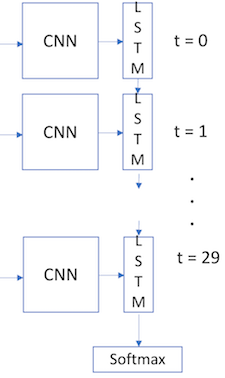
\includegraphics{architecture1.png}
\caption{alt text}
\end{figure}

To get started all you have to do is 1. Download a human action
recognition dataset (I use HMDB51)
http://serre-lab.clps.brown.edu/resource/hmdb-a-large-human-motion-database/\#Downloads
2. Create a folder called "datasets" in the root of the project
directory. 3. Put the HMDB dataset in the datasets directory, unzip it,
and rename it to "HMDB". Within the HMDB folder, unzip/unrar any actions
you want recognized. 4. Run this notebook!

You should have a directory that looks something like this:

\begin{quote}
CNN\_RNN\_Human\_Action\_Recognition/datasets/HMDB/situp/
CNN\_RNN\_Human\_Action\_Recognition/datasets/HMDB/walk/
CNN\_RNN\_Human\_Action\_Recognition/datasets/HMDB/pushup/
CNN\_RNN\_Human\_Action\_Recognition/datasets/HMDB/run/
CNN\_RNN\_Human\_Action\_Recognition/datasets/HMDB/throw/
\end{quote}

    \begin{Verbatim}[commandchars=\\\{\}]
{\color{incolor}In [{\color{incolor} }]:} \PY{k+kn}{from} \PY{n+nn}{data\PYZus{}processing}\PY{n+nn}{.}\PY{n+nn}{datasets} \PY{k}{import} \PY{o}{*}
        \PY{k+kn}{from} \PY{n+nn}{train\PYZus{}model} \PY{k}{import} \PY{n}{train\PYZus{}model}
        \PY{k+kn}{from} \PY{n+nn}{test\PYZus{}model} \PY{k}{import} \PY{n}{test\PYZus{}model}
        \PY{k+kn}{from} \PY{n+nn}{plot\PYZus{}model\PYZus{}stats} \PY{k}{import} \PY{n}{plot\PYZus{}model\PYZus{}stats}
        \PY{k+kn}{import} \PY{n+nn}{torch}
        \PY{k+kn}{import} \PY{n+nn}{torch}\PY{n+nn}{.}\PY{n+nn}{nn} \PY{k}{as} \PY{n+nn}{nn}
        \PY{k+kn}{import} \PY{n+nn}{torch}\PY{n+nn}{.}\PY{n+nn}{nn}\PY{n+nn}{.}\PY{n+nn}{functional} \PY{k}{as} \PY{n+nn}{F}
        \PY{k+kn}{import} \PY{n+nn}{torch}\PY{n+nn}{.}\PY{n+nn}{optim} \PY{k}{as} \PY{n+nn}{optim}
        \PY{k+kn}{from} \PY{n+nn}{torchvision} \PY{k}{import} \PY{n}{models}\PY{p}{,} \PY{n}{transforms}
        \PY{k+kn}{import} \PY{n+nn}{numpy} \PY{k}{as} \PY{n+nn}{np}
        \PY{k+kn}{import} \PY{n+nn}{matplotlib}\PY{n+nn}{.}\PY{n+nn}{pyplot} \PY{k}{as} \PY{n+nn}{plt}
        \PY{k+kn}{from} \PY{n+nn}{torch}\PY{n+nn}{.}\PY{n+nn}{utils}\PY{n+nn}{.}\PY{n+nn}{data}\PY{n+nn}{.}\PY{n+nn}{sampler} \PY{k}{import} \PY{n}{SubsetRandomSampler}
        \PY{n}{device} \PY{o}{=} \PY{n}{torch}\PY{o}{.}\PY{n}{device}\PY{p}{(}\PY{l+s+s2}{\PYZdq{}}\PY{l+s+s2}{cuda:0}\PY{l+s+s2}{\PYZdq{}} \PY{k}{if} \PY{n}{torch}\PY{o}{.}\PY{n}{cuda}\PY{o}{.}\PY{n}{is\PYZus{}available}\PY{p}{(}\PY{p}{)} \PY{k}{else} \PY{l+s+s2}{\PYZdq{}}\PY{l+s+s2}{cpu}\PY{l+s+s2}{\PYZdq{}}\PY{p}{)}
\end{Verbatim}


    Model Design

    \begin{Verbatim}[commandchars=\\\{\}]
{\color{incolor}In [{\color{incolor} }]:} \PY{k}{class} \PY{n+nc}{CNNLSTMNet}\PY{p}{(}\PY{n}{nn}\PY{o}{.}\PY{n}{Module}\PY{p}{)}\PY{p}{:}
            \PY{k}{def} \PY{n+nf}{\PYZus{}\PYZus{}init\PYZus{}\PYZus{}}\PY{p}{(}\PY{n+nb+bp}{self}\PY{p}{,} \PY{n}{cnn\PYZus{}model}\PY{p}{,} \PY{n}{output\PYZus{}dim}\PY{p}{,} \PY{n}{hidden\PYZus{}dim}\PY{p}{,}\PY{n}{num\PYZus{}classes}\PY{o}{=}\PY{l+m+mi}{10}\PY{p}{,}\PY{n}{seq\PYZus{}len}\PY{o}{=}\PY{l+m+mi}{20} \PY{p}{,}\PY{n}{batch\PYZus{}size}\PY{o}{=}\PY{l+m+mi}{1}\PY{p}{,} \PY{n}{num\PYZus{}lstm\PYZus{}layers} \PY{o}{=} \PY{l+m+mi}{1}\PY{p}{,} \PY{n}{bidirectional} \PY{o}{=} \PY{k+kc}{False}\PY{p}{,} \PY{n}{device} \PY{o}{=} \PY{l+s+s1}{\PYZsq{}}\PY{l+s+s1}{cpu}\PY{l+s+s1}{\PYZsq{}}\PY{p}{,} \PY{n}{freeze\PYZus{}layers}\PY{o}{=}\PY{k+kc}{True}\PY{p}{,} \PY{n}{dropout}\PY{o}{=}\PY{l+m+mi}{0}\PY{p}{,} \PY{n}{title}\PY{o}{=}\PY{l+s+s2}{\PYZdq{}}\PY{l+s+s2}{default}\PY{l+s+s2}{\PYZdq{}}\PY{p}{)}\PY{p}{:}
                \PY{n+nb}{super}\PY{p}{(}\PY{n}{CNNLSTMNet}\PY{p}{,} \PY{n+nb+bp}{self}\PY{p}{)}\PY{o}{.}\PY{n+nf+fm}{\PYZus{}\PYZus{}init\PYZus{}\PYZus{}}\PY{p}{(}\PY{p}{)}
                \PY{c+c1}{\PYZsh{} CNN}
                \PY{n+nb+bp}{self}\PY{o}{.}\PY{n}{device} \PY{o}{=} \PY{n}{device}
                \PY{n+nb+bp}{self}\PY{o}{.}\PY{n}{title} \PY{o}{=} \PY{n}{title} \PY{c+c1}{\PYZsh{} Model Title}
                \PY{n+nb+bp}{self}\PY{o}{.}\PY{n}{cnn\PYZus{}model} \PY{o}{=} \PY{n}{cnn\PYZus{}model} \PY{c+c1}{\PYZsh{} Torchvision CNN Model}
                
                \PY{c+c1}{\PYZsh{} Optionally Freeze CNN Layers}
                \PY{k}{if} \PY{n}{freeze\PYZus{}layers}\PY{p}{:}
                    \PY{k}{for} \PY{n}{idxc}\PY{p}{,} \PY{n}{child} \PY{o+ow}{in} \PY{n+nb}{enumerate}\PY{p}{(}\PY{n+nb+bp}{self}\PY{o}{.}\PY{n}{cnn\PYZus{}model}\PY{o}{.}\PY{n}{children}\PY{p}{(}\PY{p}{)}\PY{p}{)}\PY{p}{:}
                        \PY{k}{for} \PY{n}{param} \PY{o+ow}{in} \PY{n}{child}\PY{o}{.}\PY{n}{parameters}\PY{p}{(}\PY{p}{)}\PY{p}{:}
                            \PY{n}{param}\PY{o}{.}\PY{n}{requires\PYZus{}grad} \PY{o}{=} \PY{k+kc}{False}
                    \PY{n+nb+bp}{self}\PY{o}{.}\PY{n}{cnn\PYZus{}model}\PY{o}{.}\PY{n}{fc}\PY{o}{.}\PY{n}{requires\PYZus{}grad} \PY{o}{=} \PY{k+kc}{True}
                    
                \PY{c+c1}{\PYZsh{} RNN}
                \PY{n+nb+bp}{self}\PY{o}{.}\PY{n}{seq\PYZus{}len} \PY{o}{=} \PY{n}{seq\PYZus{}len}
                \PY{n+nb+bp}{self}\PY{o}{.}\PY{n}{batch\PYZus{}size} \PY{o}{=} \PY{n}{batch\PYZus{}size}
                \PY{n+nb+bp}{self}\PY{o}{.}\PY{n}{hidden\PYZus{}dim} \PY{o}{=} \PY{n}{hidden\PYZus{}dim} \PY{c+c1}{\PYZsh{} LSTM Hidden Dimension Size}
                \PY{n+nb+bp}{self}\PY{o}{.}\PY{n}{num\PYZus{}lstm\PYZus{}layers} \PY{o}{=} \PY{n}{num\PYZus{}lstm\PYZus{}layers} 
                \PY{n+nb+bp}{self}\PY{o}{.}\PY{n}{bidirectional} \PY{o}{=} \PY{n}{bidirectional} \PY{c+c1}{\PYZsh{} Sets LSTM to Uni or Bidirectional}
                \PY{n+nb+bp}{self}\PY{o}{.}\PY{n}{bidirectional\PYZus{}mult} \PY{o}{=} \PY{l+m+mi}{2} \PY{k}{if} \PY{n+nb+bp}{self}\PY{o}{.}\PY{n}{bidirectional} \PY{k}{else} \PY{l+m+mi}{1} \PY{c+c1}{\PYZsh{} Used for LSTM Weight Shape}
                \PY{n+nb+bp}{self}\PY{o}{.}\PY{n}{lstm} \PY{o}{=} \PY{n}{nn}\PY{o}{.}\PY{n}{LSTM}\PY{p}{(}\PY{n}{output\PYZus{}dim}\PY{p}{,} \PY{n}{hidden\PYZus{}dim}\PY{p}{,} \PY{n+nb+bp}{self}\PY{o}{.}\PY{n}{num\PYZus{}lstm\PYZus{}layers}\PY{p}{,} \PY{n}{bidirectional}\PY{o}{=}\PY{n+nb+bp}{self}\PY{o}{.}\PY{n}{bidirectional}\PY{p}{,} \PY{n}{dropout}\PY{o}{=}\PY{n}{dropout}\PY{p}{)}
                \PY{n+nb+bp}{self}\PY{o}{.}\PY{n}{hidden2class} \PY{o}{=} \PY{n}{nn}\PY{o}{.}\PY{n}{Linear}\PY{p}{(}\PY{n}{hidden\PYZus{}dim}\PY{o}{*}\PY{n+nb+bp}{self}\PY{o}{.}\PY{n}{bidirectional\PYZus{}mult}\PY{p}{,} \PY{n}{num\PYZus{}classes}\PY{p}{)} \PY{c+c1}{\PYZsh{} Fully Connected Output Layer}
                \PY{n+nb+bp}{self}\PY{o}{.}\PY{n}{hidden} \PY{o}{=} \PY{n+nb+bp}{self}\PY{o}{.}\PY{n}{init\PYZus{}hidden}\PY{p}{(}\PY{p}{)}
        
            \PY{k}{def} \PY{n+nf}{init\PYZus{}hidden}\PY{p}{(}\PY{n+nb+bp}{self}\PY{p}{)}\PY{p}{:}
                \PY{c+c1}{\PYZsh{} (num\PYZus{}layers, minibatch\PYZus{}size, hidden\PYZus{}dim)}
                \PY{k}{return} \PY{p}{(}\PY{n}{torch}\PY{o}{.}\PY{n}{zeros}\PY{p}{(}\PY{n+nb+bp}{self}\PY{o}{.}\PY{n}{num\PYZus{}lstm\PYZus{}layers}\PY{o}{*}\PY{n+nb+bp}{self}\PY{o}{.}\PY{n}{bidirectional\PYZus{}mult}\PY{p}{,} \PY{n+nb+bp}{self}\PY{o}{.}\PY{n}{batch\PYZus{}size}\PY{p}{,} \PY{n+nb+bp}{self}\PY{o}{.}\PY{n}{hidden\PYZus{}dim}\PY{p}{)}\PY{o}{.}\PY{n}{to}\PY{p}{(}\PY{n}{device}\PY{p}{)}\PY{p}{,}
                            \PY{n}{torch}\PY{o}{.}\PY{n}{zeros}\PY{p}{(}\PY{n+nb+bp}{self}\PY{o}{.}\PY{n}{num\PYZus{}lstm\PYZus{}layers}\PY{o}{*}\PY{n+nb+bp}{self}\PY{o}{.}\PY{n}{bidirectional\PYZus{}mult}\PY{p}{,} \PY{n+nb+bp}{self}\PY{o}{.}\PY{n}{batch\PYZus{}size}\PY{p}{,} \PY{n+nb+bp}{self}\PY{o}{.}\PY{n}{hidden\PYZus{}dim}\PY{p}{)}\PY{o}{.}\PY{n}{to}\PY{p}{(}\PY{n}{device}\PY{p}{)}\PY{p}{)}
        
        
            \PY{k}{def} \PY{n+nf}{forward}\PY{p}{(}\PY{n+nb+bp}{self}\PY{p}{,} \PY{n}{x}\PY{p}{)}\PY{p}{:}
                \PY{n}{x} \PY{o}{=} \PY{n}{x}\PY{o}{.}\PY{n}{view}\PY{p}{(}\PY{n+nb+bp}{self}\PY{o}{.}\PY{n}{seq\PYZus{}len}\PY{o}{*}\PY{n+nb+bp}{self}\PY{o}{.}\PY{n}{batch\PYZus{}size}\PY{p}{,}\PY{n}{x}\PY{o}{.}\PY{n}{shape}\PY{p}{[}\PY{o}{\PYZhy{}}\PY{l+m+mi}{3}\PY{p}{]}\PY{p}{,}\PY{n}{x}\PY{o}{.}\PY{n}{shape}\PY{p}{[}\PY{o}{\PYZhy{}}\PY{l+m+mi}{2}\PY{p}{]}\PY{p}{,}\PY{o}{\PYZhy{}}\PY{l+m+mi}{1}\PY{p}{)}
                \PY{n}{out} \PY{o}{=} \PY{n+nb+bp}{self}\PY{o}{.}\PY{n}{cnn\PYZus{}model}\PY{p}{(}\PY{n}{x}\PY{p}{)}
                \PY{n}{seq} \PY{o}{=} \PY{n}{out}\PY{o}{.}\PY{n}{view}\PY{p}{(}\PY{n+nb+bp}{self}\PY{o}{.}\PY{n}{batch\PYZus{}size}\PY{p}{,} \PY{n+nb+bp}{self}\PY{o}{.}\PY{n}{seq\PYZus{}len}\PY{p}{,} \PY{o}{\PYZhy{}}\PY{l+m+mi}{1}\PY{p}{)}\PY{o}{.}\PY{n}{transpose\PYZus{}}\PY{p}{(}\PY{l+m+mi}{0}\PY{p}{,}\PY{l+m+mi}{1}\PY{p}{)}
                \PY{n+nb+bp}{self}\PY{o}{.}\PY{n}{hidden} \PY{o}{=} \PY{n+nb+bp}{self}\PY{o}{.}\PY{n}{init\PYZus{}hidden}\PY{p}{(}\PY{p}{)}
                \PY{c+c1}{\PYZsh{} LSTM input shape = (seq\PYZus{}len, batch, input\PYZus{}size)}
                \PY{n}{out}\PY{p}{,} \PY{n+nb+bp}{self}\PY{o}{.}\PY{n}{hidden} \PY{o}{=} \PY{n+nb+bp}{self}\PY{o}{.}\PY{n}{lstm}\PY{p}{(}\PY{n}{seq}\PY{o}{.}\PY{n}{view}\PY{p}{(}\PY{n+nb}{len}\PY{p}{(}\PY{n}{seq}\PY{p}{)}\PY{p}{,} \PY{n+nb+bp}{self}\PY{o}{.}\PY{n}{batch\PYZus{}size}\PY{p}{,} \PY{o}{\PYZhy{}}\PY{l+m+mi}{1}\PY{p}{)}\PY{p}{,} \PY{n+nb+bp}{self}\PY{o}{.}\PY{n}{hidden}\PY{p}{)}
                \PY{c+c1}{\PYZsh{}LSTM output shape = (seq\PYZus{}len, batch, hidden\PYZus{}dim * bidirectional)}
                \PY{n}{out} \PY{o}{=} \PY{n+nb+bp}{self}\PY{o}{.}\PY{n}{hidden2class}\PY{p}{(}\PY{n}{out}\PY{p}{[}\PY{o}{\PYZhy{}}\PY{l+m+mi}{1}\PY{p}{]}\PY{p}{)}
                \PY{k}{return} \PY{n}{out}
\end{Verbatim}


    Display Data

    \begin{Verbatim}[commandchars=\\\{\}]
{\color{incolor}In [{\color{incolor} }]:} \PY{n}{root\PYZus{}dir}\PY{o}{=}\PY{l+s+s1}{\PYZsq{}}\PY{l+s+s1}{../datasets}\PY{l+s+s1}{\PYZsq{}}
        \PY{n}{train\PYZus{}transform} \PY{o}{=} \PY{n}{transforms}\PY{o}{.}\PY{n}{Compose}\PY{p}{(}
            \PY{p}{[}
                \PY{n}{transforms}\PY{o}{.}\PY{n}{ToPILImage}\PY{p}{(}\PY{p}{)}\PY{p}{,}
                \PY{n}{transforms}\PY{o}{.}\PY{n}{Resize}\PY{p}{(}\PY{l+m+mi}{256}\PY{p}{)}\PY{p}{,}  \PY{c+c1}{\PYZsh{} 1. Resize smallest side to 256.}
                \PY{n}{transforms}\PY{o}{.}\PY{n}{CenterCrop}\PY{p}{(}\PY{l+m+mi}{224}\PY{p}{)}\PY{p}{,} \PY{c+c1}{\PYZsh{} 2. Crop the center 224x224 pixels.}
                \PY{n}{transforms}\PY{o}{.}\PY{n}{ToTensor}\PY{p}{(}\PY{p}{)}\PY{p}{,}
                \PY{n}{transforms}\PY{o}{.}\PY{n}{Normalize}\PY{p}{(}\PY{n}{mean} \PY{o}{=} \PY{p}{[}\PY{l+m+mf}{0.485}\PY{p}{,} \PY{l+m+mf}{0.456}\PY{p}{,} \PY{l+m+mf}{0.406}\PY{p}{]}\PY{p}{,}  \PY{c+c1}{\PYZsh{} Normalize. This is necessary when using torchnet pretrained models.}
                                  \PY{n}{std} \PY{o}{=} \PY{p}{[}\PY{l+m+mf}{0.229}\PY{p}{,} \PY{l+m+mf}{0.224}\PY{p}{,} \PY{l+m+mf}{0.225}\PY{p}{]}\PY{p}{)}
            \PY{p}{]}\PY{p}{)}
        
        \PY{n}{trainset} \PY{o}{=} \PY{n}{HMDB}\PY{p}{(}\PY{l+m+mi}{30}\PY{p}{,} \PY{n}{root\PYZus{}dir}\PY{o}{=}\PY{n}{root\PYZus{}dir}\PY{p}{,} \PY{n}{transforms}\PY{o}{=}\PY{n}{train\PYZus{}transform}\PY{p}{)} \PY{c+c1}{\PYZsh{}Use ending 20 frames from each clip}
        \PY{n+nb}{print}\PY{p}{(}\PY{l+s+s2}{\PYZdq{}}\PY{l+s+s2}{Train size:}\PY{l+s+s2}{\PYZdq{}}\PY{p}{,}\PY{n+nb}{len}\PY{p}{(}\PY{n}{trainset}\PY{p}{)}\PY{p}{)}
\end{Verbatim}


    \begin{Verbatim}[commandchars=\\\{\}]
{\color{incolor}In [{\color{incolor} }]:} \PY{k}{def} \PY{n+nf}{display\PYZus{}sequence}\PY{p}{(}\PY{n}{trainset}\PY{p}{)}\PY{p}{:}
            \PY{n+nb}{print}\PY{p}{(}\PY{l+s+s1}{\PYZsq{}}\PY{l+s+s1}{Labels:}\PY{l+s+s1}{\PYZsq{}}\PY{p}{,} \PY{n}{trainset}\PY{o}{.}\PY{n}{labels}\PY{p}{)}
            
            \PY{c+c1}{\PYZsh{} Sample the dataset}
            \PY{n}{rand\PYZus{}int} \PY{o}{=} \PY{n}{np}\PY{o}{.}\PY{n}{random}\PY{o}{.}\PY{n}{randint}\PY{p}{(}\PY{l+m+mi}{0}\PY{p}{,}\PY{n+nb}{len}\PY{p}{(}\PY{n}{trainset}\PY{p}{)}\PY{p}{)}
            \PY{n}{sample\PYZus{}video}\PY{p}{,} \PY{n}{label} \PY{o}{=} \PY{n}{trainset}\PY{p}{[}\PY{n}{rand\PYZus{}int}\PY{p}{]}
            \PY{n}{video\PYZus{}label} \PY{o}{=} \PY{n}{trainset}\PY{o}{.}\PY{n}{data\PYZus{}file\PYZus{}labels}\PY{p}{[}\PY{n}{rand\PYZus{}int}\PY{p}{]}
            \PY{n}{num\PYZus{}frame} \PY{o}{=} \PY{l+m+mi}{6} \PY{c+c1}{\PYZsh{} Number of frames to display}
            
            \PY{c+c1}{\PYZsh{} Display Frames}
            \PY{n}{frames} \PY{o}{=} \PY{n}{np}\PY{o}{.}\PY{n}{asarray}\PY{p}{(}\PY{n}{transforms}\PY{o}{.}\PY{n}{ToPILImage}\PY{p}{(}\PY{p}{)}\PY{p}{(}\PY{n}{sample\PYZus{}video}\PY{p}{[}\PY{l+m+mi}{0}\PY{p}{]}\PY{p}{)}\PY{p}{)}
            \PY{n+nb}{print}\PY{p}{(}\PY{l+s+s1}{\PYZsq{}}\PY{l+s+s1}{Data Shape:}\PY{l+s+s1}{\PYZsq{}}\PY{p}{,} \PY{n}{sample\PYZus{}video}\PY{o}{.}\PY{n}{shape}\PY{p}{)}
            \PY{k}{for} \PY{n}{i} \PY{o+ow}{in} \PY{n+nb}{range}\PY{p}{(}\PY{l+m+mi}{1}\PY{p}{,} \PY{n}{trainset}\PY{o}{.}\PY{n}{seq\PYZus{}len}\PY{p}{,}\PY{n+nb}{int}\PY{p}{(}\PY{n}{trainset}\PY{o}{.}\PY{n}{seq\PYZus{}len}\PY{o}{/}\PY{n}{num\PYZus{}frame}\PY{p}{)}\PY{p}{)}\PY{p}{:}
                \PY{n}{frame} \PY{o}{=} \PY{n}{sample\PYZus{}video}\PY{p}{[}\PY{n}{i}\PY{p}{]}
                \PY{k}{for} \PY{n}{t}\PY{p}{,} \PY{n}{m}\PY{p}{,} \PY{n}{s} \PY{o+ow}{in} \PY{n+nb}{zip}\PY{p}{(}\PY{n}{frame}\PY{p}{,} \PY{p}{[}\PY{l+m+mf}{0.485}\PY{p}{,} \PY{l+m+mf}{0.456}\PY{p}{,} \PY{l+m+mf}{0.406}\PY{p}{]}\PY{p}{,} \PY{p}{[}\PY{l+m+mf}{0.229}\PY{p}{,} \PY{l+m+mf}{0.224}\PY{p}{,} \PY{l+m+mf}{0.225}\PY{p}{]}\PY{p}{)}\PY{p}{:}
                    \PY{n}{t}\PY{o}{.}\PY{n}{mul\PYZus{}}\PY{p}{(}\PY{n}{s}\PY{p}{)}\PY{o}{.}\PY{n}{add\PYZus{}}\PY{p}{(}\PY{n}{m}\PY{p}{)}
                \PY{n}{frame} \PY{o}{=} \PY{n}{np}\PY{o}{.}\PY{n}{asarray}\PY{p}{(}\PY{n}{transforms}\PY{o}{.}\PY{n}{ToPILImage}\PY{p}{(}\PY{p}{)}\PY{p}{(}\PY{n}{frame}\PY{p}{)}\PY{p}{)}
                \PY{n}{frames} \PY{o}{=} \PY{n}{np}\PY{o}{.}\PY{n}{concatenate}\PY{p}{(}\PY{p}{(}\PY{n}{frames}\PY{p}{,} \PY{n}{frame}\PY{p}{)}\PY{p}{,} \PY{n}{axis}\PY{o}{=}\PY{l+m+mi}{1}\PY{p}{)}
                \PY{n+nb}{print}\PY{p}{(}\PY{n}{i}\PY{p}{,} \PY{l+s+s2}{\PYZdq{}}\PY{l+s+s2}{frame size:}\PY{l+s+s2}{\PYZdq{}}\PY{p}{,} \PY{n}{frame}\PY{o}{.}\PY{n}{shape}\PY{p}{,} \PY{l+s+s1}{\PYZsq{}}\PY{l+s+s1}{label:}\PY{l+s+s1}{\PYZsq{}}\PY{p}{,} \PY{n}{video\PYZus{}label}\PY{p}{)}
            \PY{n+nb}{print}\PY{p}{(}\PY{l+s+s1}{\PYZsq{}}\PY{l+s+s1}{Frame sequence}\PY{l+s+s1}{\PYZsq{}}\PY{p}{)}
            \PY{n+nb}{print}\PY{p}{(}\PY{n}{frames}\PY{o}{.}\PY{n}{shape}\PY{p}{)}
            \PY{n+nb}{print}\PY{p}{(}\PY{l+s+s1}{\PYZsq{}}\PY{l+s+s1}{Visualize the data where the first image is normalized, and the rest are not.}\PY{l+s+s1}{\PYZsq{}}\PY{p}{)}
            \PY{n}{plt}\PY{o}{.}\PY{n}{figure}\PY{p}{(}\PY{n}{figsize}\PY{o}{=}\PY{p}{(}\PY{l+m+mi}{50}\PY{p}{,} \PY{l+m+mi}{10}\PY{p}{)}\PY{p}{)}
            \PY{n}{plt}\PY{o}{.}\PY{n}{grid}\PY{p}{(}\PY{k+kc}{False}\PY{p}{)}\PY{p}{;}
            \PY{n}{plt}\PY{o}{.}\PY{n}{imshow}\PY{p}{(}\PY{n}{frames}\PY{p}{)}
        
        
        \PY{n}{display\PYZus{}sequence}\PY{p}{(}\PY{n}{trainset}\PY{p}{)}
\end{Verbatim}


    Model Variables

    \begin{Verbatim}[commandchars=\\\{\}]
{\color{incolor}In [{\color{incolor} }]:} \PY{n}{num\PYZus{}img\PYZus{}features} \PY{o}{=} \PY{l+m+mi}{1024} \PY{c+c1}{\PYZsh{} CNN output dimensions}
        \PY{n}{num\PYZus{}epochs} \PY{o}{=} \PY{l+m+mi}{10}
        \PY{n}{sequence\PYZus{}len} \PY{o}{=} \PY{n}{trainset}\PY{o}{.}\PY{n}{seq\PYZus{}len} \PY{c+c1}{\PYZsh{} LSTM sequence length}
        \PY{n}{batch\PYZus{}size}\PY{o}{=}\PY{l+m+mi}{3}
        \PY{n}{hidden\PYZus{}dim} \PY{o}{=} \PY{l+m+mi}{128} \PY{c+c1}{\PYZsh{} LSTM hidden dimension size}
        \PY{n}{lstm\PYZus{}dropout} \PY{o}{=} \PY{o}{.}\PY{l+m+mi}{1}
        \PY{n}{lstm\PYZus{}depth} \PY{o}{=} \PY{l+m+mi}{1}
        \PY{n}{freeze} \PY{o}{=} \PY{k+kc}{False} \PY{c+c1}{\PYZsh{} True = Freeze entire CNN, False = Don\PYZsq{}t freeze any layers}
        \PY{n}{pretrain} \PY{o}{=} \PY{k+kc}{True} \PY{c+c1}{\PYZsh{} Use Imagenet Pretraining with CNN}
        \PY{n}{lstm\PYZus{}depth\PYZus{}title} \PY{o}{=} \PY{l+s+s1}{\PYZsq{}}\PY{l+s+s1}{no\PYZus{}freeze\PYZus{}layers\PYZus{}num\PYZus{}lstm\PYZus{}layers\PYZus{}}\PY{l+s+s1}{\PYZsq{}}\PY{o}{+}\PY{n+nb}{str}\PY{p}{(}\PY{n}{lstm\PYZus{}depth}\PY{p}{)}
        \PY{n}{num\PYZus{}classes} \PY{o}{=} \PY{n+nb}{len}\PY{p}{(}\PY{n}{trainset}\PY{o}{.}\PY{n}{labels}\PY{p}{)}
        \PY{n}{loss\PYZus{}fn} \PY{o}{=} \PY{n}{nn}\PY{o}{.}\PY{n}{CrossEntropyLoss}\PY{p}{(}\PY{p}{)}
        
        
        \PY{n}{title} \PY{o}{=}\PYZbs{}
        \PY{l+s+s1}{\PYZsq{}}\PY{l+s+s1}{\PYZhy{}dataset\PYZhy{}}\PY{l+s+s1}{\PYZsq{}}\PY{o}{+}\PY{n+nb}{str}\PY{p}{(}\PY{n}{trainset}\PY{o}{.}\PY{n}{title}\PY{p}{)}\PY{o}{+}\PYZbs{}
        \PY{l+s+s1}{\PYZsq{}}\PY{l+s+s1}{\PYZhy{}frozen\PYZhy{}}\PY{l+s+s1}{\PYZsq{}}\PY{o}{+}\PY{n+nb}{str}\PY{p}{(}\PY{n}{freeze}\PY{p}{)}\PY{o}{+}\PYZbs{}
        \PY{l+s+s1}{\PYZsq{}}\PY{l+s+s1}{\PYZhy{}num\PYZus{}img\PYZus{}features\PYZhy{}}\PY{l+s+s1}{\PYZsq{}}\PY{o}{+} \PY{n+nb}{str}\PY{p}{(}\PY{n}{num\PYZus{}img\PYZus{}features}\PY{p}{)} \PY{o}{+}\PYZbs{}
        \PY{l+s+s1}{\PYZsq{}}\PY{l+s+s1}{\PYZhy{}num\PYZus{}epochs\PYZhy{}}\PY{l+s+s1}{\PYZsq{}}\PY{o}{+}\PY{n+nb}{str}\PY{p}{(}\PY{n}{num\PYZus{}epochs}\PY{p}{)}\PY{o}{+}\PYZbs{}
        \PY{l+s+s1}{\PYZsq{}}\PY{l+s+s1}{\PYZhy{}sequence\PYZus{}len\PYZhy{}}\PY{l+s+s1}{\PYZsq{}}\PY{o}{+}\PY{n+nb}{str}\PY{p}{(}\PY{n}{sequence\PYZus{}len}\PY{p}{)}\PY{o}{+}\PYZbs{}
        \PY{l+s+s1}{\PYZsq{}}\PY{l+s+s1}{\PYZhy{}batch\PYZus{}size\PYZhy{}}\PY{l+s+s1}{\PYZsq{}}\PY{o}{+}\PY{n+nb}{str}\PY{p}{(}\PY{n}{batch\PYZus{}size}\PY{p}{)}\PY{o}{+}\PYZbs{}
        \PY{l+s+s1}{\PYZsq{}}\PY{l+s+s1}{\PYZhy{}lstm\PYZus{}dim\PYZhy{}}\PY{l+s+s1}{\PYZsq{}}\PY{o}{+}\PY{n+nb}{str}\PY{p}{(}\PY{n}{hidden\PYZus{}dim}\PY{p}{)}\PY{o}{+}\PYZbs{}
        \PY{l+s+s1}{\PYZsq{}}\PY{l+s+s1}{\PYZhy{}lstm\PYZus{}depth\PYZhy{}}\PY{l+s+s1}{\PYZsq{}}\PY{o}{+}\PY{n+nb}{str}\PY{p}{(}\PY{n}{lstm\PYZus{}depth}\PY{p}{)}\PY{o}{+}\PYZbs{}
        \PY{l+s+s1}{\PYZsq{}}\PY{l+s+s1}{\PYZhy{}pretrain\PYZhy{}}\PY{l+s+s1}{\PYZsq{}}\PY{o}{+}\PY{n+nb}{str}\PY{p}{(}\PY{n}{pretrain}\PY{p}{)}\PY{o}{+}\PYZbs{}
        \PY{l+s+s1}{\PYZsq{}}\PY{l+s+s1}{CNN\PYZhy{}resnet18}\PY{l+s+s1}{\PYZsq{}}
\end{Verbatim}


    ResNet18 + Unidirectional LSTM

    \begin{Verbatim}[commandchars=\\\{\}]
{\color{incolor}In [{\color{incolor} }]:} \PY{n}{cnn\PYZus{}model} \PY{o}{=} \PY{n}{models}\PY{o}{.}\PY{n}{resnet18}\PY{p}{(}\PY{n}{pretrained}\PY{o}{=}\PY{n}{pretrain}\PY{p}{)} \PY{c+c1}{\PYZsh{}Choose different CNN if desired}
        \PY{n}{num\PYZus{}ftrs} \PY{o}{=} \PY{n}{cnn\PYZus{}model}\PY{o}{.}\PY{n}{fc}\PY{o}{.}\PY{n}{in\PYZus{}features}
        \PY{n}{cnn\PYZus{}model}\PY{o}{.}\PY{n}{fc} \PY{o}{=} \PY{n}{nn}\PY{o}{.}\PY{n}{Linear}\PY{p}{(}\PY{n}{num\PYZus{}ftrs}\PY{p}{,} \PY{n}{num\PYZus{}img\PYZus{}features}\PY{p}{)} \PY{c+c1}{\PYZsh{} Change CNN output layer to desired dimension}
        \PY{n}{model} \PY{o}{=} \PY{n}{CNNLSTMNet}\PY{p}{(}\PY{n}{cnn\PYZus{}model}\PY{p}{,} \PY{n}{num\PYZus{}img\PYZus{}features}\PY{p}{,} \PY{n}{hidden\PYZus{}dim}\PY{p}{,} \PY{n}{num\PYZus{}classes}\PY{p}{,} \PY{n}{sequence\PYZus{}len}\PY{p}{,} \PY{n}{batch\PYZus{}size}\PY{p}{,} \PY{n}{num\PYZus{}lstm\PYZus{}layers}\PY{o}{=}\PY{n}{lstm\PYZus{}depth}\PY{p}{,} \PY{n}{bidirectional}\PY{o}{=}\PY{k+kc}{False}\PY{p}{,} \PY{n}{device}\PY{o}{=}\PY{n}{device}\PY{p}{,} \PY{n}{freeze\PYZus{}layers}\PY{o}{=}\PY{n}{freeze}\PY{p}{,} \PY{n}{dropout}\PY{o}{=}\PY{n}{lstm\PYZus{}dropout}\PY{p}{)}
        \PY{n}{optimizer} \PY{o}{=} \PY{n}{optim}\PY{o}{.}\PY{n}{Adam}\PY{p}{(}\PY{n}{model}\PY{o}{.}\PY{n}{parameters}\PY{p}{(}\PY{p}{)}\PY{p}{,} \PY{n}{lr} \PY{o}{=} \PY{l+m+mf}{1e\PYZhy{}4}\PY{p}{)}
        \PY{n}{model\PYZus{}save\PYZus{}path}\PY{o}{=} \PY{l+s+s1}{\PYZsq{}}\PY{l+s+s1}{saved\PYZus{}models/}\PY{l+s+s1}{\PYZsq{}}\PY{o}{+}\PY{n}{title}\PY{o}{+}\PY{l+s+s1}{\PYZsq{}}\PY{l+s+s1}{.pth}\PY{l+s+s1}{\PYZsq{}}
        \PY{c+c1}{\PYZsh{} Use Below to load train history and train over a saved model}
        \PY{c+c1}{\PYZsh{} model.load\PYZus{}state\PYZus{}dict(torch.load(model\PYZus{}save\PYZus{}path))}
        \PY{n+nb}{print}\PY{p}{(}\PY{n}{title}\PY{p}{)}
\end{Verbatim}


    \begin{Verbatim}[commandchars=\\\{\}]
{\color{incolor}In [{\color{incolor} }]:} \PY{n}{train\PYZus{}model}\PY{p}{(}\PY{n}{model}\PY{p}{,} \PY{n}{loss\PYZus{}fn}\PY{p}{,} \PY{n}{batch\PYZus{}size}\PY{p}{,} \PY{n}{trainset}\PY{p}{,} \PY{n}{optimizer}\PY{p}{,} \PY{n}{title}\PY{p}{,} \PY{n}{device}\PY{p}{,} \PY{n}{num\PYZus{}epochs}\PY{o}{=}\PY{n}{num\PYZus{}epochs}\PY{p}{)}
\end{Verbatim}



    % Add a bibliography block to the postdoc
    
    
    
    \end{document}
